\section{Results}\label{sec:results}

Table~\ref{tab:verdicts} summarises the verdicts. Sections~\ref{sec:res-rq1}--\ref{sec:res-rq4} report the pre-specified analyses, and Section~\ref{sec:res-robust} reports the robustness checks that were added after the main results.

\begin{table*}[t]
\centering\footnotesize
\caption{Hypotheses and verdicts. Evidence marked $\dagger$ comes from post hoc robustness checks (Section~\ref{sec:res-robust}).}
\label{tab:verdicts}
\begin{tabular}{@{}l>{\raggedright}p{3.2cm}>{\raggedright\arraybackslash}p{12.6cm}@{}}
\toprule
Hyp. & Verdict & Key evidence\\
\midrule
H1 & Supported, with exceptions & Relatedness $+0.10$ TR per step ($p<.001$), also with corpus terms and the fertility gap$^\dagger$. A sister-language source from the target's corpus beats the same language from the other corpus on isiZulu news ($+32.0$~F1) and isiXhosa news ($+12.7$; both Holm $p=.005$), and on isiZulu government text ($+8.2$, not tested), but not on isiXhosa or Setswana government text\\
H2 & Not supported & Seen targets have neither higher F1 nor higher TR, and exposure is not significant ($p=.19$--$.36$). Exposure is confounded with cluster and fertility, so the result is inconclusive and not negative\\
H3 & Supported & 500 target sentences close 57--89\% of every gap. Most of the gain arrives by 100 sentences only for the two weakest starting points\\
H4 & Rejected (reversed) & Swahili beats Sepedi and Sesotho on Setswana news by 14.3 and 19.0~F1, and Sepedi on Setswana government text by 13.0 (two-sided Holm $p=.01$). The gap is unchanged with equal entity counts$^\dagger$\\
\bottomrule
\end{tabular}
\end{table*}

\subsection{RQ1: Relatedness versus domain match}\label{sec:res-rq1}
Relatedness is the most consistent predictor of zero-shot transfer (Figures~\ref{fig:heatmap} and~\ref{fig:rq1}). Same-language and same-cluster sources average 56--61~F1, against 37--47 for sources from other clusters, and at every relatedness level a source from the test set's own corpus adds only 0.04--0.08 to the transfer ratio. In M0, relatedness adds $+0.10$ to the transfer ratio per step ($p<.001$, 95\% CI 0.05--0.15), whereas neither the domain-match term ($p=.71$) nor its interaction with relatedness ($p=.79$) is significant.

In contrast, the pre-specified contrasts show where corpus match overrides relatedness (Table~\ref{tab:rq1}). On both news targets, a sister-language news source beats a same-language government source, by 32.0~F1 for isiZulu and by 12.7 for isiXhosa (both Holm $p=.005$, and positive in every seed). On government targets the picture is mixed: the sister-language government source also wins for isiZulu ($+8.2$), but the same-language news source wins for isiXhosa ($+21.4$) and Setswana ($+5.6$ to $+13.4$). Furthermore, transfer inside NCHLT is uneven, since isiZulu and isiXhosa reach only 46--52~F1 on each other's NCHLT test sets, against about 83 on news, where our sister-pair results match MasakhaNER~2.0 (82.4 vs 82.1; 82.7 vs 83.7, with a different model)~\cite{adelani2022}.

\begin{figure}[t]
\centering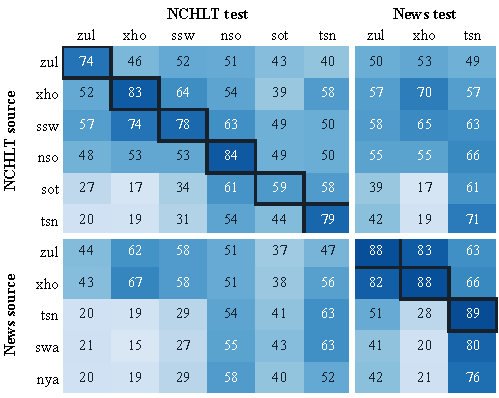
\includegraphics[width=\columnwidth]{figures/zero_shot_heatmap}
\caption{Zero-shot F1 for all source--test pairs (mean of 3 seeds, rounded). Rows are sources and columns are test sets; in-language cells are outlined.}
\label{fig:heatmap}
\end{figure}

\begin{figure}[t]
\centering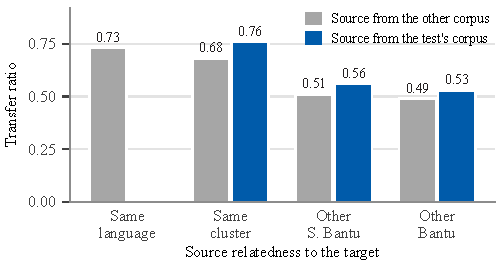
\includegraphics[width=\columnwidth]{figures/rq1_relatedness_corpus}
\caption{RQ1: mean transfer ratio by source relatedness and by whether the source comes from the test set's corpus (seed-level transfer pairs). A same-language source is always from the other corpus.}
\label{fig:rq1}
\end{figure}

\begin{table}[t]
\centering\footnotesize
\caption{RQ1: sister language in the same corpus vs same language in the other corpus (F1, mean of 3 seeds). $^*$Pre-specified, Holm $p=.005$.}
\label{tab:rq1}
\begin{tabular}{@{}lllr@{}}
\toprule
Test & Sister, same corpus & Same lang., other & $\Delta$\\
\midrule
zul news & xho news 82.4 & zul govt 50.4 & $+32.0^*$\\
xho news & zul news 82.7 & xho govt 70.0 & $+12.7^*$\\
zul govt & xho govt 52.4 & zul news 44.2 & $+8.2$\\
xho govt & zul govt 45.9 & xho news 67.3 & $-21.4$\\
tsn govt & nso govt 49.9 & tsn news 63.3 & $-13.4$\\
tsn govt & sot govt 57.7 & tsn news 63.3 & $-5.6$\\
\bottomrule
\end{tabular}
\end{table}

\paragraph{H1 verdict} Supported, with exceptions. Relatedness is the stronger general predictor; however, matching the target's corpus overrides it in three of the six comparisons, including both pre-specified news contrasts. Since each corpus has its own annotation guideline, this ``domain'' effect may come from the text, the labels or both.

\subsection{RQ2: Pretraining exposure}\label{sec:res-rq2}
Unseen targets score as high as or higher than seen targets at every relatedness level (Table~\ref{tab:rq2}), and the in-language NCHLT scores are highest for unseen Sepedi (83.6) and lowest for seen Sesotho (59.5). Exposure is not significant in any regression ($p=.19$--$.36$). In fact, from distant (other-Bantu) sources the transfer ratio is higher for unseen targets (0.66 against 0.38). However, two of the three unseen targets are Sotho-Tswana languages, which accept low-fertility sources such as Swahili well; therefore, exposure, cluster and fertility move together, and the anomalous Sesotho corpus lowers the seen group.

\begin{table}[t]
\centering\footnotesize
\caption{RQ2: mean zero-shot F1 by source relatedness and target exposure. The unseen same-language cell has one language (Setswana).}
\label{tab:rq2}
\begin{tabular}{@{}lrr@{}}
\toprule
Source relatedness & Seen targets & Unseen targets\\
\midrule
Same language (other corpus) & 58.0 & 67.0\\
Same cluster & 57.7 & 57.8\\
Other Southern Bantu & 35.1 & 50.8\\
Other Bantu & 28.2 & 55.1\\
\bottomrule
\end{tabular}
\end{table}

\paragraph{H2 verdict} Not supported. With six targets, exposure cannot be separated from cluster, fertility and corpus quality, so the absence of an advantage is inconclusive and not evidence against exposure.

\subsection{RQ3: Few-shot target data}\label{sec:res-rq3}
With 500 target sentences every gap narrows (Figure~\ref{fig:rq3}, Table~\ref{tab:rq3}), and 57--89\% of the gap to the in-language model closes. Government sources nearly catch up with sister-language news sources (isiZulu 83.5 vs 86.2; isiXhosa 83.6 vs 85.8), and for Setswana the Sepedi source (85.1) slightly passes the Setswana government source (84.0). The shape of the curves differs from the common finding that most of the gain arrives by 100 sentences~\cite{lauscher2020}. This holds only for the two sources furthest from the target (75\% and 62\%), whereas near-ceiling sources gain mainly between 100 and 500 sentences, and the isiZulu news source for isiXhosa does not improve at all by 100 sentences. For those sources the total gain is only 3--4~F1, which is close to seed variation, so their shares are imprecise.

\begin{figure*}[t]
\centering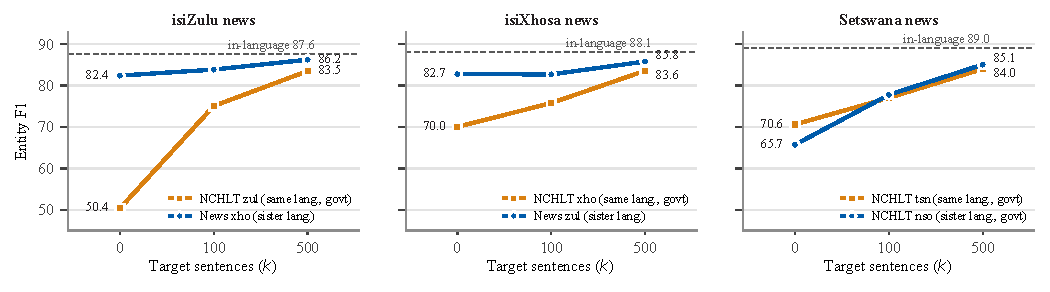
\includegraphics[width=\textwidth]{figures/rq3_fewshot_curves}
\caption{RQ3: few-shot learning curves on the three news targets (mean of 3 seeds). Orange: the same language from the government corpus; blue: a sister language. The dashed line is the in-language model.}
\label{fig:rq3}
\end{figure*}

\begin{table}[t]
\centering\footnotesize
\caption{RQ3: few-shot F1 (mean of 3 seeds) and share of the 500-sentence gain reached by $k=100$.}
\label{tab:rq3}
\begin{tabular}{@{}lrrrr@{}}
\toprule
Source \ra\ target & $k=0$ & $k=100$ & $k=500$ & By 100\\
\midrule
NCHLT zul \ra\ zul news & 50.4 & 75.1 & 83.5 & 75\%\\
NCHLT nso \ra\ tsn news & 65.7 & 77.8 & 85.1 & 62\%\\
NCHLT tsn \ra\ tsn news & 70.6 & 77.0 & 84.0 & 48\%\\
NCHLT xho \ra\ xho news & 70.0 & 75.8 & 83.6 & 42\%\\
News xho \ra\ zul news & 82.4 & 83.9 & 86.2 & 38\%\\
News zul \ra\ xho news & 82.7 & 82.7 & 85.8 & $-2$\%\\
\bottomrule
\end{tabular}
\end{table}

\paragraph{H3 verdict} Supported. 500 target sentences narrow every transfer gap, and they do so most quickly for weak, cross-corpus starting points.

\subsection{RQ4: Sources for Setswana}\label{sec:res-rq4}
H4 is rejected (Figure~\ref{fig:rq4}, Table~\ref{tab:rq4}). On Setswana news, Swahili (80.0) outperforms Sepedi (65.7) and Sesotho (61.0) in all three pre-specified contrasts, by 13.0--19.0~F1 and in every seed, and Chichewa (76.3) also scores above both, although no Chichewa contrast was pre-specified. The one-sided tests in the hypothesised direction give $p=1.0$, while the two-sided Holm $p$ is .01 for each contrast. Swahili is also the best other-language source on the Setswana government test (62.9). Since every Sotho-Tswana source is government text and every distant-Bantu source is news, the comparison confounds relatedness with corpus. Within NCHLT, where the corpus is fixed, Sepedi (49.9) and Sesotho (57.7) are no better than isiXhosa (57.7) on Setswana. Swahili lands well above the best published single-source scores for Setswana (73.1--73.3, with a different model and setting)~\cite{adelani2022}, and Sepedi lands below them.

\begin{figure*}[t]
\centering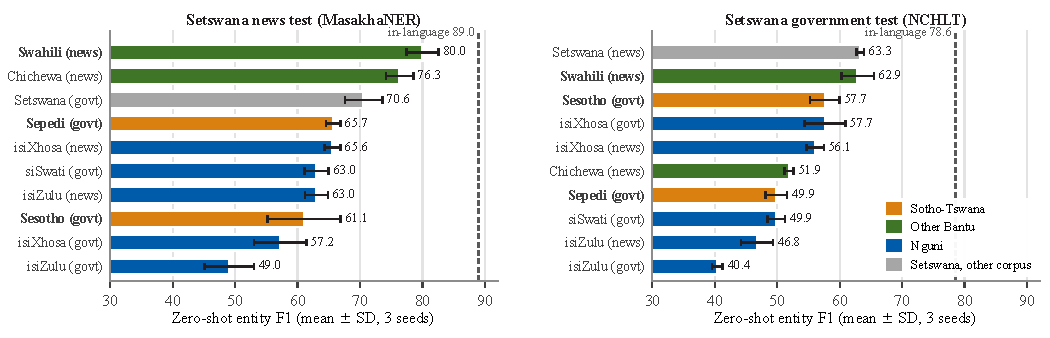
\includegraphics[width=\textwidth]{figures/rq4_setswana_sources}
\caption{RQ4: zero-shot F1 of every source on the two Setswana test sets (mean $\pm$ SD over 3 seeds), coloured by the source's language group. The three pre-specified sources are in bold; the dashed line is the in-language model.}
\label{fig:rq4}
\end{figure*}

\begin{table}[t]
\centering\footnotesize
\caption{RQ4: F1 on the two Setswana test sets with the 3,000-sentence cap and ($\dagger$, post hoc, Section~\ref{sec:res-robust}) with every source capped at 2,500 entity spans.}
\label{tab:rq4}
\begin{tabular}{@{}lrrrr@{}}
\toprule
& \multicolumn{2}{c}{News test} & \multicolumn{2}{c}{Govt test}\\
\cmidrule(lr){2-3}\cmidrule(l){4-5}
Source & sent.\ cap & ent.\ cap$^\dagger$ & sent.\ cap & ent.\ cap$^\dagger$\\
\midrule
Swahili (news) & \textbf{80.0} & 78.5 & 62.9 & 61.2\\
Chichewa (news) & 76.3 & 73.2 & 51.9 & 49.0\\
Sepedi (govt) & 65.7 & 64.2 & 49.9 & 48.7\\
Sesotho (govt) & 61.0 & 61.4 & 57.7 & 54.6\\
isiXhosa (govt) & 57.2 & 60.5 & 57.7 & 58.1\\
Setswana, other corpus & 70.6 & -- & \textbf{63.3} & --\\
\midrule
Setswana, in-language & 89.0 & -- & 78.6 & --\\
\bottomrule
\end{tabular}
\end{table}

\paragraph{H4 verdict} Rejected. On Setswana news, Swahili is a stronger source than Sepedi and Sesotho, and Chichewa also scores above both.

\subsection{Robustness checks}\label{sec:res-robust}
These checks were added after the main results and are not part of the Holm family.

\paragraph{Entity density and truncation} We re-trained the RQ4 sources on about 2,500 PER/LOC/ORG spans each (3 seeds; Table~\ref{tab:rq4}). The Swahili--Sepedi gap on Setswana news stays at 14.3~F1 (12.5 on government text), although Swahili reaches it from about half as many sentences (about 1,360 against 2,470). Furthermore, at 128 subword tokens at most 2.8\% of gold entities are truncated (NCHLT Setswana), and none are truncated in the news test sets.

\paragraph{Corpus terms and fertility} Replacing domain match in M0 with a source-corpus term and its interaction with the test corpus (M1) shows that a news source does not help government targets ($+0.016$, $p=.70$), but adds about 0.11--0.14 TR on news targets ($p=.12$; $p=.049$ once the fertility gap is added in M2). The fertility gap, which is the absolute difference in subwords per word between source and target, is the strongest added predictor ($-0.177$ TR per unit, $p=.001$; AIC $-71.2\rightarrow-78.8$), and it absorbs about a third of the relatedness coefficient ($0.112\rightarrow0.078$), which stays significant. Fertility and cluster are partly collinear; however, fertility fits an asymmetry that orthography does not. Swahili and Chichewa are written conjunctively like the Nguni languages, yet they transfer well to Sotho-Tswana targets, and Swahili's fertility (1.51) is close to that of the Sotho-Tswana corpora (about 1.8). Since the models have no source random intercept, the $p$-values of these source-level terms are likely optimistic.
